\documentclass{beamer}
\usepackage{HECbeamer}

\usepackage{icomma}
\usepackage{numprint}
\title[\color{white}{MATH 60604 \S~5f - Autres modèles de covariance}]{\texorpdfstring{MATH 60604 \\Modélisation statistique \\ \S~5f - Autres modèles de covariance}{MATH 60604 \\Modélisation statistique \\ \S~5f - Autres modèles de covariance}}
\author{}
\institute{HEC Montréal\\
Département de sciences de la décision}
\date{} 

\begin{document}
\frame{\titlepage}
\begin{frame}[fragile]
\frametitle{Choix de la structure de covariance: autres possibilités}
\bi
\item Avec des données longitudinales, il arrive parfois que la variance des
observations varie en fonction du temps de mesure. 
\item Plusieurs des structures
de covariance possibles dans la procédure \texttt{mixed} possèdent aussi une
version hétérogène, c'est-à-dire une version où les variances peuvent être
distinctes pour les différents temps de mesure. 
\item Par exemple, la structure
$\mathsf{AR}(1)$ que nous venons de voir possèdent une version hétérogène, appelée
$\mathsf{ARH}(1)$, dont la structure de covariance est
\[
\bs{\Sigma}_i=
  \begin{pmatrix}
   \sigma^2_1 & \sigma_1\sigma_2\rho & \sigma_1\sigma_3\rho^2 & \sigma_1\sigma_4\rho^3 & \sigma_1\sigma_5\rho^4\\
    \sigma_2\sigma_1\rho & \sigma^2_2 & \sigma_2\sigma_3\rho & \sigma_2\sigma_4\rho^2 & \sigma_2\sigma_5\rho^3\\
    \sigma_3\sigma_1\rho^2 & \sigma_3\sigma_2\rho & \sigma_3^2 & \sigma_3\sigma_4\rho & \sigma_3\sigma_5\rho^2\\
       \sigma_4\sigma_1\rho^3 & \sigma_4\sigma_2\rho^2 & \sigma_4\sigma_3\rho & \sigma^2_4 & \sigma_4\sigma_5\rho\\
       \sigma_5\sigma_1\rho^4 & \sigma_5\sigma_2\rho^3 & \sigma_5\sigma_3\rho^2 & \sigma_5\sigma_2\rho & \sigma_5^2
  \end{pmatrix}.
\]
\item Mais au lieu de supposer une variance commune $\sigma^2$ à tous les temps de
mesure, on suppose plutôt que la variance au temps $j$ est $\sigma^2_j$.
\ei
\end{frame}


\begin{frame}[fragile]
\frametitle{Syntaxe pour l'ajustement du modèle $\mathsf{ARH}(1)$}
 
\begin{tcolorbox}[colback=white, colframe=hecblue, title=Code \SASlang{} pour ajuster le modèle $\mathsf{ARH}(1)$]
\begin{verbatim}
proc mixed data=vengeance method=reml;
class id tcat;
model vengeance = sexe age vc wom t / solution;
repeated tcat / subject=id type=arh(1) r=1 rcorr=1;
run;
\end{verbatim}
\end{tcolorbox}

\end{frame}

\begin{frame}[fragile]
\frametitle{Matrice de corrélation et de covariance pour le sujet 1}
\begin{center}
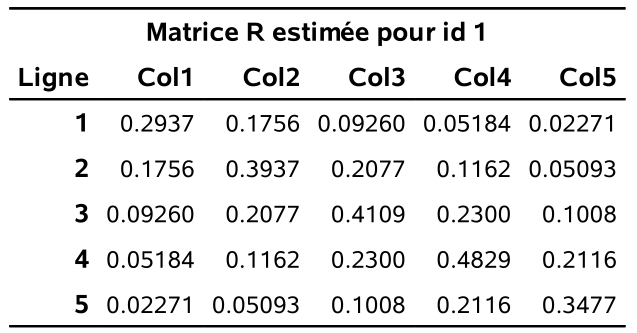
\includegraphics[width = 0.45\linewidth]{img/c5/diapos6-e18a}
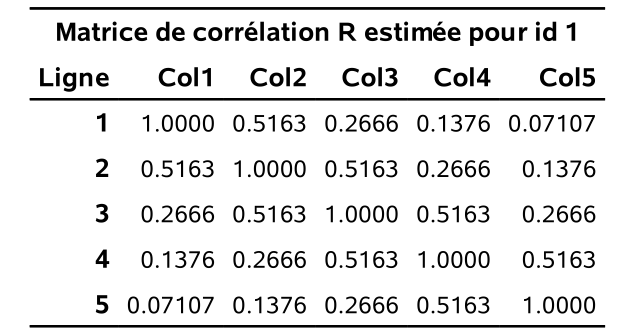
\includegraphics[width = 0.45\linewidth]{img/c5/diapos6-e18b}
\end{center}
\bi
\item La matrice de covariance montre bien que la variance des observations est différente pour chaque temps de mesure
\item la matrice de corrélation montre, comme pour la structure $\mathsf{AR}(1)$, que la corrélation entre 2 observation décroit avec le temps.
\ei
\end{frame}

\begin{frame}[fragile]
\frametitle{Estimés des paramètres de covariance du modèle $\mathsf{ARH}(1)$}
\begin{center}
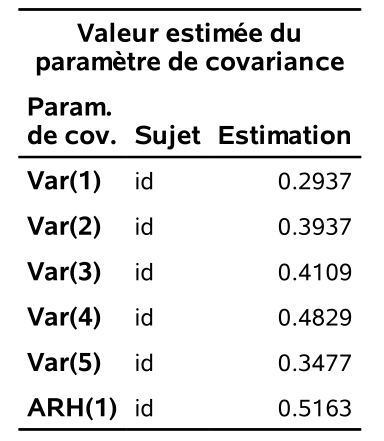
\includegraphics[width = 0.4\linewidth]{img/c5/diapos6-e19}
\end{center}
\bi
\item Ce modèle comporte six paramètres pour la structure de covariance. 
\item Dans le tableau, on voit les estimations des
variances pour les cinq unités de temps.
\item L'estimation du paramètre $\rho$ est $\hat{\rho} = \numprint{0.516}$, très semblable à celui du modèle précédent ($ \numprint{0.492}$).
\ei 
\end{frame}
% 
% 
% \begin{frame}[fragile]
% \frametitle{Exemple vengeance: sortie SAS}
% \textbf{AIC/BIC du modèle}
% \begin{center}
% \includegraphics[scale=0.35]{Figures/long30.pdf}
% \includegraphics[scale=0.35]{Figures/long31.pdf}
% %\includegraphics[scale=0.35]{Figures/long32.pdf}\\
% %\includegraphics[scale=0.35]{Figures/long33.pdf}
% \end{center}
% \bi
% \item Les AIC et BIC pourront être utilisé pour comparer les modèles avec différentes structures de corrélation
% \item Le test de LRT teste l'hypothèse que tous les coefficients $\beta$ du modèle sont nuls. Les résultats montrent que l'hypothèse nulle est rejetée.
% \ei
% \end{frame}
% 
% \begin{frame}[fragile]
% \frametitle{Exemple vengeance: sortie SAS}
% \textbf{Estimation des effets fixes du modèle}
% \begin{center}
% \includegraphics[scale=0.3]{Figures/long32.pdf}
% \includegraphics[scale=0.3]{Figures/long33.pdf}
% \end{center}
% \bi
% \item Les estimations
% des paramètres $\beta$ sont encore une fois très semblables à ceux des modèles
% précédents. 
% \item La variables \code{sexe} est sur la frontière (p-value=0.0499) quant
% au fait d'être significative ou non.
% \ei
% \end{frame}
% 


\begin{frame}[fragile]
\frametitle{Test du rapport de vraisemblance pour le modèle $\mathsf{ARH}(1)$}
\begin{center}
% 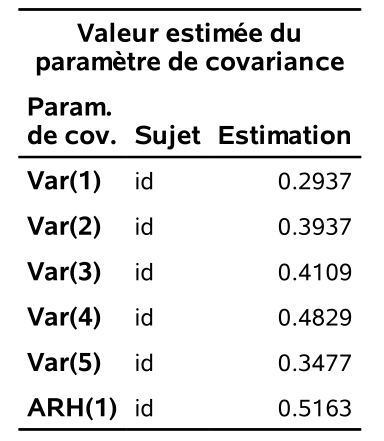
\includegraphics[width = 0.45\linewidth]{img/c5/diapos6-e19}
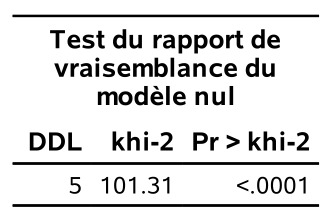
\includegraphics[width = 0.35\linewidth]{img/c5/diapos6-e20}
\end{center}
\bi
\item La sortie \SASlang{} inclut les résultats du test de rapport de vraisemblance comparant le modèle $\mathsf{ARH}(1)$ (modèle complet) au modèle homoscédastique sans corrélation (modèle réduit).
\item Les hypothèses de ce test sont $\Hy_0: \rho=0, \sigma_1^2=\sigma_2^2=\cdots=\sigma_5^2$ et  $\Hy_1: \rho \neq 0$ ou au moins une des variances différente.
\item La valeur-$p$ est négligeable et on rejette $\Hy_0$; on conclut en faveur de l'utilisation de la structure de covariance $\mathsf{ARH}(1)$.
\ei
\end{frame}

\begin{frame}[fragile]
\frametitle{Choix de la structure de covariance: autre possibilité}
\bi
\item Une autre possibilité serait de ne spécifier aucune structure pour la covariance et estimer tous les paramètres du modèle
\[
\bs{\Sigma}_i=
  \begin{pmatrix}
  \sigma^2_1 & \sigma_{12} & \sigma_{13} & \sigma_{14} & \sigma_{15} \\
   \sigma_{21} & \sigma_2^2  & \sigma_{23} & \sigma_{24} & \sigma_{25}\\
  \sigma_{31} & \sigma_{32} & \sigma^2_3 & \sigma_{34} & \sigma_{35}\\
   \sigma_{41} & \sigma_{42} & \sigma_{43} & \sigma_{4}^2 & \sigma_{45}\\
    \sigma_{51} & \sigma_{52} & \sigma_{53} & \sigma_{54}^2 & \sigma_{5}^2\\
    \end{pmatrix}
\]

\item Cette structure peut parfois être utile pour explorer la structure de covariance
sans imposer un modèle rigide dès le départ. Mais son nombre de paramètres, $n_i(n_i-1)/2$, restreint son utilisation aux cas où le nombre maximum d'observations par groupe est petit et le nombre de groupes $m$ est grand.
\item Dans notre exemple, on obtient $15$ paramètres contrairement à deux pour les structures d'équicorrélation et $\mathsf{AR}(1)$, et à
six pour la structure $\mathsf{ARH}(1)$. 
\ei
\end{frame}

\begin{frame}[fragile]
\frametitle{Ajustement du modèle de covariance non structuré}
 
\begin{tcolorbox}[colback=white, colframe=hecblue, title=Code \SASlang{} pour ajuster un modèle non structuré]
\begin{verbatim}
proc mixed data=vengeance method=reml;
class id tcat;
model vengeance = sexe age vc wom t / solution;
repeated tcat / subject=id type=un r=1 rcorr=1;
run;
\end{verbatim}
\end{tcolorbox}
\end{frame}


\begin{frame}
\frametitle{Matrice de corrélation et de covariance pour le sujet 1}
\begin{center}
%\includegraphics[scale=0.35]{Figures/long34.pdf}
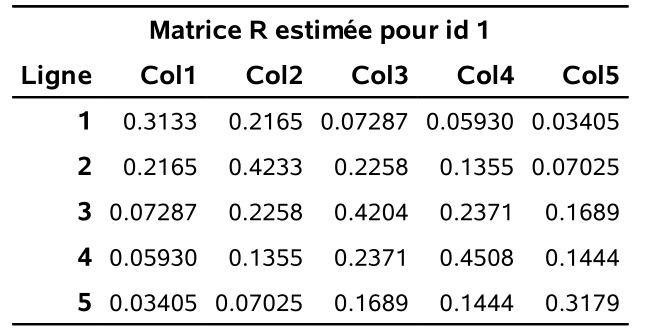
\includegraphics[width = 0.45\linewidth]{img/c5/diapos6-e21a}
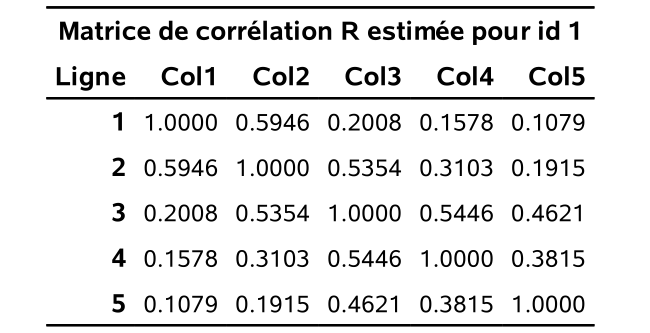
\includegraphics[width = 0.45\linewidth]{img/c5/diapos6-e21b}
\end{center}
\bi
\item On voit que les variances sont différentes pour chaque temps et il n'y a pas de structure spéciales pour la corrélation.
\be

\item Les variances semblent être à peu près les mêmes pour les mesures. 
\item La corrélation entre deux observations semble bel et bien
décroître au fur et à mesure que le temps entre deux mesures augmente. 
\ee
\item Ceci suggère que la structure $\mathsf{AR}(1)$ est préférable à la structure d'équicorrélation.
\ei
\end{frame}

\begin{frame}
\frametitle{Paramètres de covariance du modèle non structuré}
\begin{center}
%\includegraphics[scale=0.35]{Figures/long36.pdf}
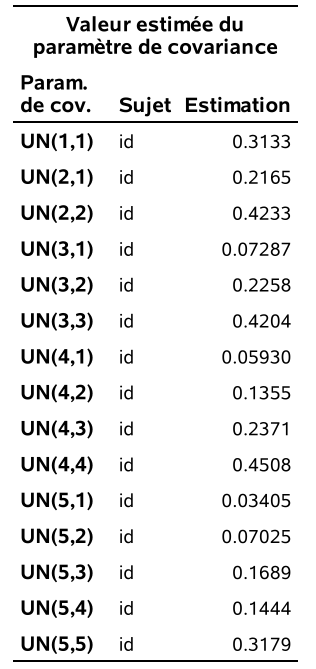
\includegraphics[width = 0.30\linewidth]{img/c5/diapos6-e22}
\end{center}

\end{frame}

\begin{frame}
\frametitle{Critères d'information et test du rapport de vraisemblance}

\begin{center}
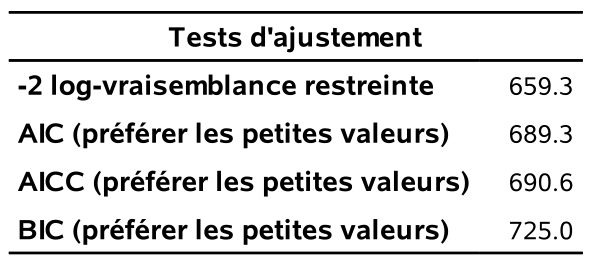
\includegraphics[width = 0.5\linewidth]{img/c5/diapos6-e23}
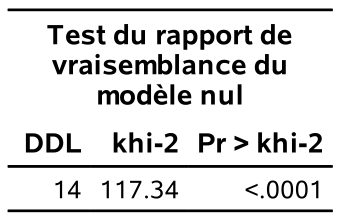
\includegraphics[width = 0.3\linewidth]{img/c5/diapos6-e24}

\end{center}
\bi
\item Comme d'ordinaire, la sortie inclut les critères \AIC{} et \BIC{}, que l'on pourra utiliser pour comparer les modèles de covariance non emboîtés.
\item Le test du rapport de vraisemblance teste l'hypothèse nulle que tous les paramètres de variance (diagonale) sont égaux et que tous les termes hors diagonale sont nuls. Cette hypothèse est rejetée.
\ei
\end{frame}
\end{document}
